\definecolor{paperInk}{HTML}{111827}
\definecolor{paperMuted}{HTML}{6B7280}
\definecolor{paperLine}{HTML}{CBD5E1}
\definecolor{paperBlue}{HTML}{2563EB}
\definecolor{paperGreen}{HTML}{059669}
\definecolor{paperOrange}{HTML}{D97706}
\definecolor{paperRed}{HTML}{DC2626}
\definecolor{paperFill}{HTML}{F8FAFC}

\tikzset{
  paperBox/.style={
    draw=paperLine,
    fill=paperFill,
    rounded corners=2pt,
    line width=0.5pt,
    align=center,
    inner sep=4pt,
    text=paperInk
  },
  paperArrow/.style={-Latex, line width=0.7pt, draw=paperInk!70},
  paperNote/.style={font=\scriptsize, text=paperMuted, align=center}
}

\pgfplotsset{
  paperAxis/.style={
    width=\linewidth,
    height=5.2cm,
    axis line style={draw=paperInk!60},
    tick style={draw=paperInk!60},
    tick label style={font=\scriptsize, text=paperInk},
    label style={font=\small, text=paperInk},
    grid=both,
    major grid style={draw=paperLine!65, line width=0.3pt},
    minor grid style={draw=paperLine!35, line width=0.2pt},
    legend style={
      font=\scriptsize,
      draw=paperLine,
      fill=white,
      rounded corners=1pt
    },
    legend cell align={left}
  }
}

\newcommand{\figWorkflow}{%
\begin{figure}[H]
  \centering
  \resizebox{\linewidth}{!}{%
  \begin{tikzpicture}[font=\small, node distance=6mm and 8mm]
    \node[paperBox, minimum width=2.25cm, minimum height=1.05cm] (raw)
      {\textbf{PIPPA}\\ShareGPT records};
    \node[paperBox, right=of raw, minimum width=2.35cm, minimum height=1.05cm] (process)
      {\textbf{Process}\\cards + turns};
    \node[paperBox, right=of process, minimum width=2.45cm, minimum height=1.05cm] (train)
      {\textbf{Assistant-only}\\4-bit QLoRA};
    \node[paperBox, right=of train, minimum width=2.30cm, minimum height=1.05cm] (generate)
      {\textbf{Generate}\\three systems};
    \node[paperBox, right=of generate, minimum width=2.30cm, minimum height=1.05cm] (judge)
      {\textbf{Judge}\\MiniMax-M3};
    \node[paperBox, right=of judge, minimum width=2.20cm, minimum height=1.05cm] (ci)
      {\textbf{Compare}\\paired 95\% CI};

    \draw[paperArrow] (raw) -- (process);
    \draw[paperArrow] (process) -- (train);
    \draw[paperArrow] (train) -- (generate);
    \draw[paperArrow] (generate) -- (judge);
    \draw[paperArrow] (judge) -- (ci);

    \node[paperBox, fill=paperBlue!6, below=8mm of generate, xshift=-2.35cm,
      minimum width=1.95cm, minimum height=0.72cm] (baseSys) {\base};
    \node[paperBox, fill=paperGreen!7, right=6mm of baseSys,
      minimum width=1.95cm, minimum height=0.72cm] (cardSys) {\card};
    \node[paperBox, fill=paperOrange!8, right=6mm of cardSys,
      minimum width=1.95cm, minimum height=0.72cm] (loraSys) {\lora};

    \node[draw=paperBlue!45, rounded corners=2pt, line width=0.5pt,
      fit=(baseSys)(cardSys)(loraSys), inner sep=5pt,
      label={[paperNote]below:decoded systems}] (systems) {};

    \draw[paperArrow] (generate.south) -- (systems.north);
    \draw[paperArrow] (systems.north east) -- (judge.south);

    \node[paperNote, above=2mm of train] {frozen base weights; train adapter only};
    \node[paperNote, below=2mm of ci] {single-turn and four-turn role-play scores};
  \end{tikzpicture}}
  \caption{Overall workflow. The same filtered evaluation prompts are decoded
  by \base, \card, and \lora, judged anonymously, and summarized with paired
  confidence intervals.}
  \label{fig:workflow}
\end{figure}%
}

\newcommand{\figLoraInjection}{%
\begin{figure}[H]
  \centering
  \resizebox{0.95\linewidth}{!}{%
  \begin{tikzpicture}[font=\small, node distance=8mm and 9mm]
    \node[paperBox, fill=paperBlue!6, minimum width=2.55cm,
      minimum height=1.05cm] (input) {input hidden\\state $x$};
    \node[paperBox, right=of input, fill=paperFill, minimum width=2.75cm,
      minimum height=1.25cm] (w0) {frozen\\$W_0$};
    \node[paperBox, right=of w0, fill=paperGreen!7, minimum width=2.50cm,
      minimum height=1.05cm] (sum) {$W_0x + BAx$};
    \node[paperBox, right=of sum, fill=paperBlue!6, minimum width=2.45cm,
      minimum height=1.05cm] (out) {adapted\\projection};

    \node[paperBox, below=9mm of w0, fill=paperOrange!8, minimum width=1.65cm,
      minimum height=0.80cm] (a) {$A$\\down};
    \node[paperBox, right=7mm of a, fill=paperOrange!8, minimum width=1.65cm,
      minimum height=0.80cm] (b) {$B$\\up};
    \node[paperBox, right=7mm of b, fill=paperOrange!8, minimum width=1.85cm,
      minimum height=0.80cm] (delta) {$\Delta W = BA$};

    \draw[paperArrow] (input) -- (w0);
    \draw[paperArrow] (w0) -- (sum);
    \draw[paperArrow] (sum) -- (out);
    \draw[paperArrow] (input.south) |- (a.west);
    \draw[paperArrow] (a) -- node[paperNote, above] {$r=8$} (b);
    \draw[paperArrow] (b) -- (delta);
    \draw[paperArrow] (delta.north) -- (sum.south);

    \node[draw=paperBlue!45, rounded corners=2pt, line width=0.5pt,
      fit=(w0), inner sep=8pt,
      label={[paperNote]above:4-bit Qwen2.5-3B weights}] {};
    \node[draw=paperOrange!70, rounded corners=2pt, line width=0.5pt,
      fit=(a)(b)(delta), inner sep=8pt,
      label={[paperNote]below:trainable LoRA path}] {};

    \node[paperBox, fill=white, above=8mm of sum, minimum width=3.25cm]
      {injected into\\\texttt{q\_proj}, \texttt{k\_proj},\\
      \texttt{v\_proj}, \texttt{o\_proj}};
    \node[paperNote, below=5mm of delta, text width=4.2cm]
      {3,686,400 trainable parameters, 0.1193\% of the base model};
  \end{tikzpicture}}
  \caption{LoRA injection schematic. The base attention projection is frozen,
  while a low-rank update path is trained for the selected Qwen2.5 attention
  projections.}
  \label{fig:lora-injection}
\end{figure}%
}

\newcommand{\figPairedEffects}{%
\begin{figure}[H]
  \centering
  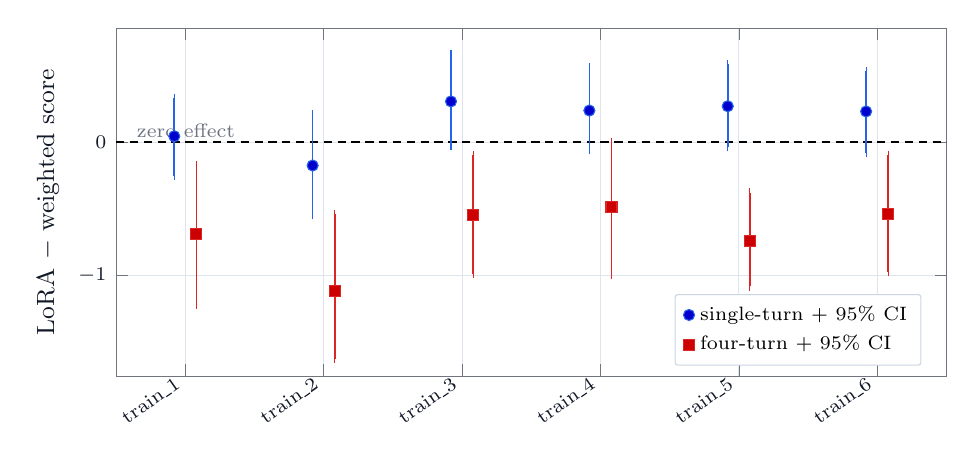
\begin{tikzpicture}
    \begin{axis}[
      paperAxis,
      height=6.0cm,
      xmin=0.5, xmax=6.5,
      ymin=-1.75, ymax=0.85,
      xtick={1,2,3,4,5,6},
      xticklabels={train\_1,train\_2,train\_3,train\_4,train\_5,train\_6},
      x tick label style={rotate=35, anchor=east, font=\scriptsize},
      ylabel={LoRA $-$ \card weighted score},
      legend pos=south east
    ]
      \addplot[black, densely dashed, line width=0.5pt, forget plot]
        coordinates {(0.5,0) (6.5,0)};
      \addplot+[
        only marks,
        mark=*,
        mark size=2.0pt,
        color=paperBlue,
        error bars/.cd,
        y dir=both,
        y explicit,
        error bar style={line width=0.6pt},
        error mark options={mark size=1.5pt}
      ] table[row sep=\\, x=x, y=y, y error plus=plus, y error minus=minus] {
        x y plus minus\\
        0.92 0.043 0.287 0.298\\
        1.92 -0.176 0.383 0.371\\
        2.92 0.303 0.353 0.332\\
        3.92 0.235 0.323 0.295\\
        4.92 0.267 0.313 0.306\\
        5.92 0.228 0.302 0.313\\
      };
      \addlegendentry{single-turn + 95\% CI}
      \addplot+[
        only marks,
        mark=square*,
        mark size=2.0pt,
        color=paperRed,
        error bars/.cd,
        y dir=both,
        y explicit,
        error bar style={line width=0.6pt},
        error mark options={mark size=1.5pt}
      ] table[row sep=\\, x=x, y=y, y error plus=plus, y error minus=minus] {
        x y plus minus\\
        1.08 -0.685 0.508 0.533\\
        2.08 -1.113 0.571 0.510\\
        3.08 -0.545 0.445 0.440\\
        4.08 -0.485 0.480 0.508\\
        5.08 -0.743 0.365 0.337\\
        6.08 -0.540 0.445 0.432\\
      };
      \addlegendentry{four-turn + 95\% CI}
      \node[anchor=west, font=\scriptsize, text=paperMuted]
        at (axis cs:0.58,0.08) {zero effect};
    \end{axis}
  \end{tikzpicture}
  \caption{Paired effects across six runs. Single-turn intervals cross zero,
  while all four-turn mean differences are negative against the prompted base
  model.}
  \label{fig:paired-effects}
\end{figure}%
}

\newcommand{\figRepetitionDiversity}{%
\begin{figure}[H]
  \centering
  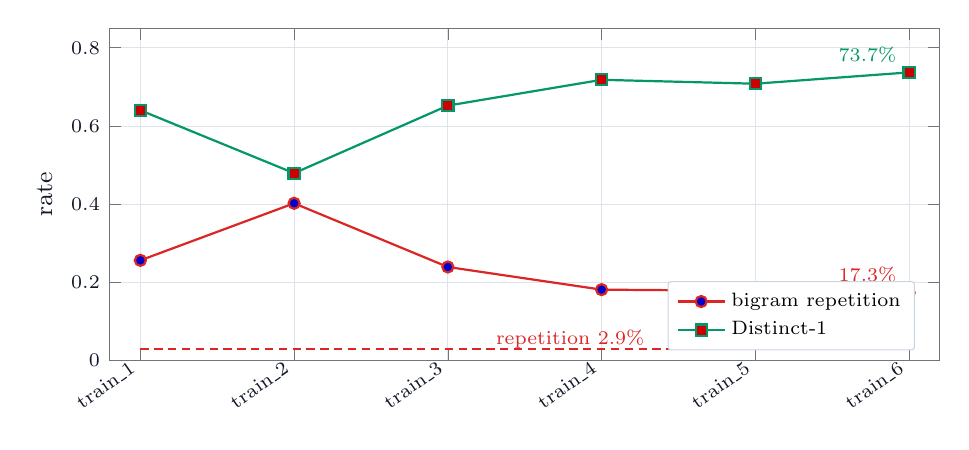
\begin{tikzpicture}
    \begin{axis}[
      paperAxis,
      height=5.8cm,
      xmin=0.8, xmax=6.2,
      ymin=0, ymax=0.85,
      xtick={1,2,3,4,5,6},
      xticklabels={train\_1,train\_2,train\_3,train\_4,train\_5,train\_6},
      x tick label style={rotate=35, anchor=east, font=\scriptsize},
      ylabel={rate},
      legend pos=south east
    ]
      \addplot+[
        color=paperRed,
        line width=0.8pt,
        mark=*,
        mark size=2.0pt
      ] coordinates {
        (1,0.256) (2,0.402) (3,0.239) (4,0.181) (5,0.178) (6,0.173)
      };
      \addlegendentry{bigram repetition}
      \addplot+[
        color=paperGreen,
        line width=0.8pt,
        mark=square*,
        mark size=2.0pt
      ] coordinates {
        (1,0.640) (2,0.479) (3,0.652) (4,0.718) (5,0.708) (6,0.737)
      };
      \addlegendentry{Distinct-1}
      \addplot[paperRed, densely dashed, line width=0.5pt, forget plot]
        coordinates {(1,0.029) (6,0.029)};
      \node[anchor=west, font=\scriptsize, text=paperRed]
        at (axis cs:3.25,0.055) {\card repetition 2.9\%};
      \node[anchor=south east, font=\scriptsize, text=paperRed]
        at (axis cs:5.98,0.173) {17.3\%};
      \node[anchor=south east, font=\scriptsize, text=paperGreen]
        at (axis cs:5.98,0.737) {73.7\%};
    \end{axis}
  \end{tikzpicture}
  \caption{Repetition and diversity trend. Later LoRA runs reduce repetition
  and recover Distinct-1, but train\_6 still has 17.3\% repetition, far above
  the 2.9\% \card baseline observed in train\_4.}
  \label{fig:repetition-diversity}
\end{figure}%
}
